\chapter{Implementação}
\label{textuais/cap5}

% ---------------------------------------------------------------------
% Marcadores usados neste capítulo:
%  \preencher{...}            -> dado que só o autor tem (aparece em vermelho no PDF)
%  \figuraprovisoria{alt}{..} -> espaço reservado para foto ou captura de tela;
%                                troque pela linha \includegraphics indicada no comentário
% ---------------------------------------------------------------------
\providecommand{\preencher}[1]{\textcolor{red}{[#1]}}
\providecommand{\figuraprovisoria}[2]{\fbox{\parbox[c][#1][c]{0.9\textwidth}{\centering\textcolor{red}{#2}}}}

Este capítulo descreve como o sistema especificado no Capítulo~\ref{textuais/cap4} foi construído. A Seção~\ref{sec:arquitetura} apresenta a arquitetura geral e a divisão do código entre as três aplicações. As seções seguintes detalham cada camada: o hardware do dispositivo de campo (Seção~\ref{sec:hardware}), o firmware e a lógica de irrigação (Seção~\ref{sec:firmware}), a API (Seção~\ref{sec:backend}) e o painel web (Seção~\ref{sec:frontend}).

% =====================================================================
\section{Arquitetura do sistema}
\label{sec:arquitetura}

O sistema segue a arquitetura em quatro camadas apresentada na fundamentação teórica \cite{morchid2024}, como mostra a Figura~\ref{fig:arquitetura}. Na camada de percepção, o ESP32 lê os sensores e aciona a válvula. Na camada de rede, ele se comunica com a API por Wi-Fi, usando HTTPS. Na camada de nuvem, a API em Spring Boot aplica as regras do sistema e guarda os dados no Cloud Firestore. Na camada de aplicação, o painel web em Angular apresenta as informações ao usuário e envia seus comandos.

\begin{figure}[htbp]
  \centering
  \begin{tikzpicture}[
      font=\footnotesize,
      camada/.style={draw, dashed, rounded corners=3pt, inner sep=5pt},
      bloco/.style={draw, rounded corners=2pt, align=center, fill=white, minimum height=1.0cm},
      rotulo/.style={font=\scriptsize\bfseries, anchor=south west, inner sep=1pt},
      seta/.style={-{Stealth[length=2mm]}, thick},
      dupla/.style={{Stealth[length=2mm]}-{Stealth[length=2mm]}, thick},
      msg/.style={font=\scriptsize, align=center, inner sep=1pt}
    ]
    % Percepção
    \node[bloco, text width=2.4cm] (sens) at (0, 0.75) {Sensores\\ \scriptsize umidade do solo e DHT11};
    \node[bloco, text width=2.4cm] (atua) at (0,-0.75) {Atuadores\\ \scriptsize relé, válvula e LCD};
    \node[bloco, text width=1.6cm, minimum height=2.5cm] (esp) at (3.3,0) {ESP32\\ \scriptsize firmware};
    \draw[seta] (sens.east) -- (sens.east -| esp.west);
    \draw[seta] (atua.east -| esp.west) -- (atua.east);
    % Nuvem
    \node[bloco, text width=2.4cm, minimum height=2.5cm] (api) at (8.0,0) {API REST\\ \scriptsize Java 17 e Spring Boot};
    \node[bloco, text width=2.4cm] (fs) at (8.0, 2.35) {Cloud Firestore};
    \node[bloco, text width=2.4cm] (auth) at (8.0,-2.35) {Firebase Authentication};
    % Aplicação
    \node[bloco, text width=2.0cm, minimum height=2.5cm] (front) at (12.2,0) {Painel web\\ \scriptsize Angular};
    % Fluxos
    \draw[seta] ([yshift=6mm]esp.east) -- node[msg, above] {leituras, estado\\ e histórico} ([yshift=6mm]api.west);
    \draw[seta] ([yshift=-6mm]api.west) -- node[msg, below] {comandos\\ (long-polling)} ([yshift=-6mm]esp.east);
    \draw[dupla] (api.north) -- (fs.south);
    \draw[dupla] (api.south) -- (auth.north);
    \draw[seta] ([yshift=6mm]api.east) -- node[msg, above] {dados} ([yshift=6mm]front.west);
    \draw[seta] ([yshift=-6mm]front.west) -- node[msg, below] {comandos} ([yshift=-6mm]api.east);
    \draw[seta, dashed] (front.south) |- node[msg, pos=0.25, right] {login} (auth.east);
    % Camadas
    \node[camada, fit=(sens)(atua)(esp)] (cp) {};
    \node[rotulo] at (cp.north west) {Percepção};
    \node[camada, fit=(api)(fs)(auth)] (cn) {};
    \node[rotulo] at (cn.north west) {Nuvem};
    \node[camada, fit=(front)] (ca) {};
    \node[rotulo] at (ca.north west) {Aplicação};
    \node[msg, font=\scriptsize\bfseries] at ($(esp.east)!0.5!(api.west) + (0,2.05)$) {Rede\\ (Wi-Fi e HTTPS)};
  \end{tikzpicture}
  \caption{Arquitetura geral do sistema}
  \label{fig:arquitetura}
  \fonte{Elaborado pelo autor}
\end{figure}

Os dados circulam em dois sentidos. No sentido do campo para o painel, o ESP32 envia as leituras, o seu estado e o registro de cada irrigação à API, que os grava no Firestore; o painel consulta a API periodicamente e exibe os dados atualizados. No sentido inverso, cada ação do usuário no painel, como trocar o modo ou iniciar uma irrigação, é enviada à API, que a transforma em um comando e o entrega ao ESP32 na próxima consulta do dispositivo. Assim, o dispositivo nunca recebe conexões de fora: ele sempre inicia a comunicação, o que dispensa configurar a rede local para aceitar acessos externos.

O código está dividido em três aplicações independentes, cada uma organizada em pacotes, como mostra a Figura~\ref{fig:pacotes}. O firmware separa a leitura dos sensores, o acionamento dos atuadores, as regras de irrigação e a comunicação; a API separa controladores, serviços, repositórios, modelos e segurança; e o painel separa os serviços e modelos compartilhados das telas. Essa divisão atende ao requisito de manutenibilidade (RNF12) e permite alterar uma parte sem modificar as demais.

\begin{figure}[htbp]
  \centering
  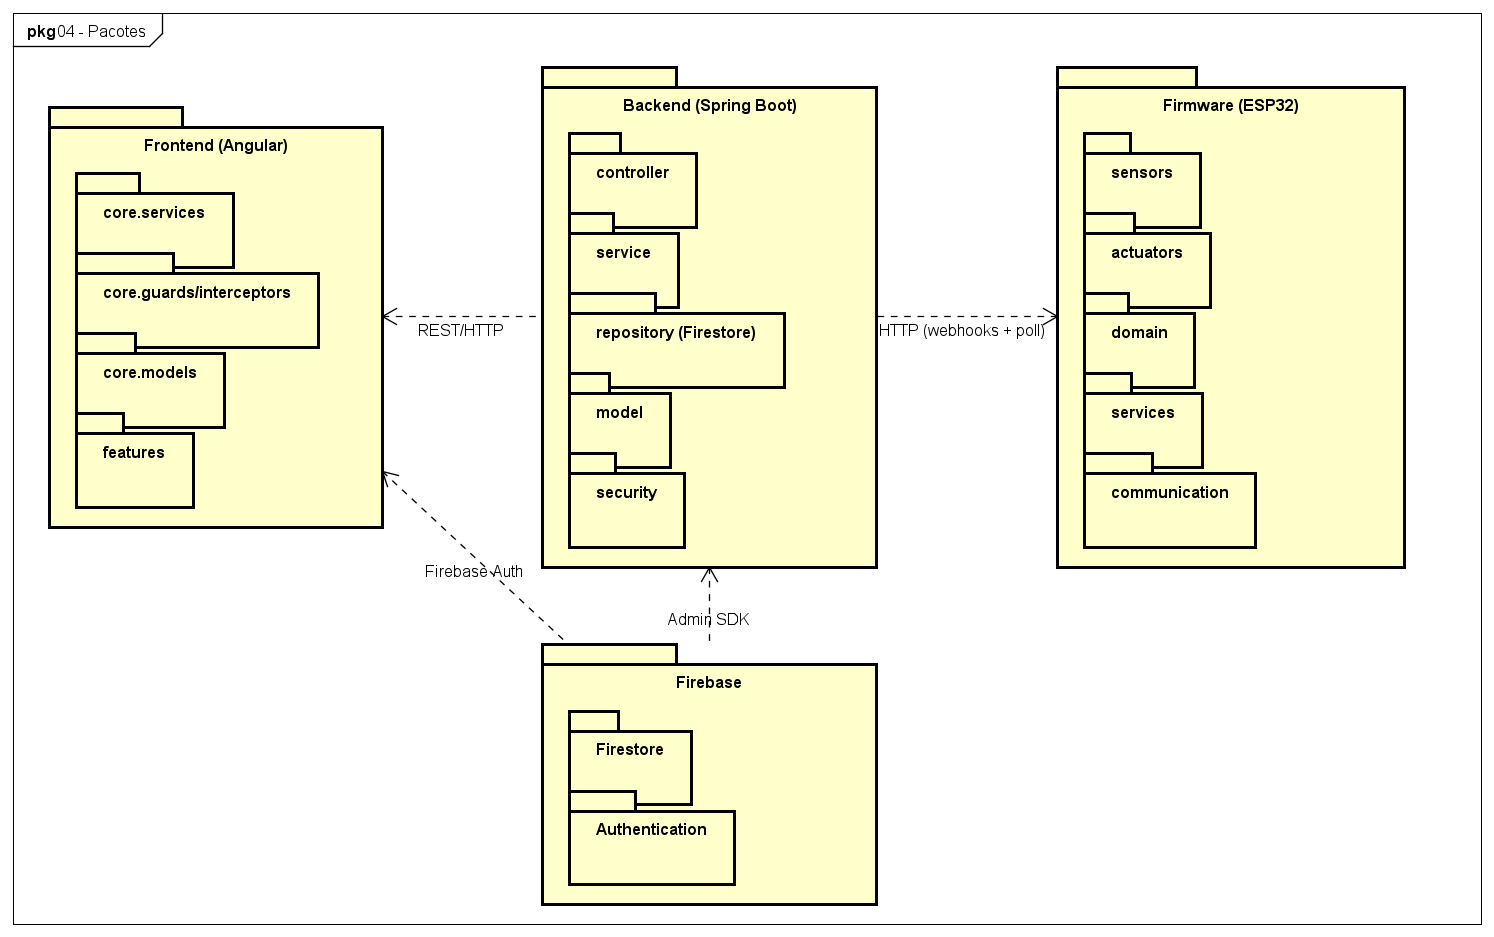
\includegraphics[width=\textwidth]{figuras/Diagrama de Pacotes.png}
  \caption{Diagrama de pacotes do sistema}
  \label{fig:pacotes}
  \fonte{Elaborado pelo autor}
\end{figure}

% =====================================================================
\section{Hardware}
\label{sec:hardware}

O dispositivo de campo é formado pelos componentes descritos na fundamentação teórica e listados na Tabela~\ref{tab:componentes}. O ESP32 concentra a leitura dos sensores, o cálculo da irrigação e a comunicação com a API. O sensor de umidade do solo é do tipo resistivo e é ligado a uma entrada analógica do ESP32; o DHT11 usa um pino digital; o display LCD 16x2 se comunica pelo barramento I2C; e o módulo relé, ligado a uma saída digital, abre e fecha o circuito de 12~V da válvula solenoide.

\begin{table}[htbp]
  \centering
  \caption{Componentes do dispositivo de campo}
  \label{tab:componentes}
  \small
  \renewcommand{\arraystretch}{1.2}
  \begin{tabularx}{\textwidth}{>{\raggedright\arraybackslash}p{4.2cm}
                               >{\raggedright\arraybackslash}X
                               >{\centering\arraybackslash}p{1.2cm}
                               >{\raggedleft\arraybackslash}p{2.2cm}}
    \hline
    \textbf{Componente} & \textbf{Função} & \textbf{Qtd.} & \textbf{Custo (R\$)} \\
    \hline
    ESP32 DevKit & Leitura dos sensores, cálculo e comunicação Wi-Fi & 1 & \preencher{valor} \\
    Sensor de umidade do solo resistivo & Umidade do solo, por entrada analógica & 1 & \preencher{valor} \\
    DHT11 & Temperatura e umidade do ar & 1 & \preencher{valor} \\
    Módulo relé & Acionamento da válvula & 1 & \preencher{valor} \\
    Válvula solenoide 12~V & Liberação da água para o gotejamento & 1 & \preencher{valor} \\
    Display LCD 16x2 com módulo I2C & Exibição local das leituras e do estado & 1 & \preencher{valor} \\
    Fonte de 12~V & Alimentação da válvula & 1 & \preencher{valor} \\
    \preencher{alimentação do ESP32} & \preencher{ex.: regulador de tensão ou fonte USB de 5~V} & 1 & \preencher{valor} \\
    Fios, conectores e protoboard & Ligações & -- & \preencher{valor} \\
    Mangueira e gotejadores & Distribuição da água & \preencher{qtd.} & \preencher{valor} \\
    \hline
    \multicolumn{3}{r}{\textbf{Total}} & \preencher{valor} \\
    \hline
  \end{tabularx}
  \fonte{Elaborado pelo autor, com preços consultados em \preencher{lojas} em \preencher{mês/ano}}
\end{table}

A Tabela~\ref{tab:ligacoes} indica os pinos do ESP32 usados por cada componente, e a Figura~\ref{fig:esquema} apresenta o esquema de ligação. O sensor de umidade do solo foi ligado ao GPIO 34, que pertence ao primeiro conversor analógico-digital (ADC1) do ESP32, porque o segundo conversor (ADC2) não pode ser usado enquanto o Wi-Fi está ativo. O display usa os pinos padrão do barramento I2C no ESP32, e o relé começa desligado assim que o pino é configurado. A válvula e o ESP32 trabalham com tensões diferentes, por isso a válvula é alimentada por uma fonte própria de 12~V, e apenas o sinal de controle do relé sai do ESP32.

\begin{table}[htbp]
  \centering
  \caption{Ligações dos componentes ao ESP32}
  \label{tab:ligacoes}
  \small
  \renewcommand{\arraystretch}{1.2}
  \begin{tabularx}{\textwidth}{>{\raggedright\arraybackslash}p{4.2cm}
                               >{\raggedright\arraybackslash}p{3.6cm}
                               >{\raggedright\arraybackslash}X}
    \hline
    \textbf{Componente} & \textbf{Pino do ESP32} & \textbf{Tipo de sinal} \\
    \hline
    Sensor de umidade do solo & GPIO 34 & Analógico (ADC1, 12 bits) \\
    DHT11 & GPIO 27 & Digital, um fio \\
    Display LCD (SDA / SCL) & GPIO 21 / GPIO 22 & I2C, endereço 0x27 \\
    Módulo relé & GPIO 26 & Saída digital \\
    \hline
  \end{tabularx}
  \fonte{Elaborado pelo autor}
\end{table}

\begin{figure}[htbp]
  \centering
  % Troque a linha abaixo por: \includegraphics[width=\textwidth]{figuras/esquema-eletrico}
  \figuraprovisoria{7cm}{Inserir o esquema de ligação dos componentes ao ESP32 (ex.: feito no Fritzing)}
  \caption{Esquema de ligação do dispositivo de campo}
  \label{fig:esquema}
  \fonte{Elaborado pelo autor}
\end{figure}

% =====================================================================
\section{Firmware e lógica de irrigação}
\label{sec:firmware}

O firmware foi escrito em C++ com o framework Arduino para o ESP32, usando as bibliotecas DHT sensor library, LiquidCrystal\_I2C e ArduinoJson. Ele preserva a lógica de cálculo do primeiro protótipo e a organiza em módulos com responsabilidades separadas. A classe IrrigationState guarda o estado do dispositivo (modo, autorização, volume de água, temperaturas mínima e máxima, irrigação em andamento e latitude) e os parâmetros agronômicos (ConfigIrrigacao). O módulo IrrigationService concentra as regras de irrigação; o IrrigationRunner controla o relé durante uma irrigação; o CommandPoller recebe os comandos da API; e o ApiClient faz todas as chamadas HTTP. Os módulos SoilSensor, DhtSensor, Relay e Display encapsulam o acesso ao hardware.

\subsection{Funcionamento geral}
\label{subsec:firmware-ciclo}

Ao ser ligado, o dispositivo mantém o relé desligado, conecta-se ao Wi-Fi, sincroniza o relógio por NTP no fuso de Brasília e busca na API a sua configuração inicial: modo, autorização, latitude e parâmetros agronômicos. Se a API não responder, o firmware segue com valores padrão locais, conforme a regra RN22. A partir daí, o trabalho é dividido entre tarefas concorrentes do FreeRTOS, sistema operacional de tempo real usado pelo ESP32. Três tarefas ficam ativas o tempo todo: a sensorTask lê os sensores e envia os dados, a statusSyncTask envia o estado do dispositivo e a commandPollTask aguarda os comandos da API. Uma quarta tarefa, a irrigationTask, é criada no início de cada irrigação e encerrada ao fim dela, o que garante que só exista uma irrigação por vez. Como as tarefas leem e alteram o mesmo estado, o acesso a ele é protegido por um mutex, que impede que duas tarefas o modifiquem ao mesmo tempo (RNF08).

A tarefa de leitura lê os sensores a cada 10~s, atualiza as temperaturas mínima e máxima do dia, mostra os valores no display e envia a telemetria à API. A cada 20~s, a statusSyncTask envia o estado completo do dispositivo. Quando um envio falha, o módulo ApiClient repete a tentativa com intervalos crescentes, até cinco vezes; esgotadas as tentativas, a leitura é descartada para não travar a tarefa (RNF07). A Figura~\ref{fig:fluxograma} resume o ciclo de funcionamento e a decisão de irrigar.

\begin{figure}[htbp]
  \centering
  \begin{tikzpicture}[
      node distance=5mm and 8mm,
      font=\footnotesize,
      passo/.style={draw, rounded corners=2pt, align=center, text width=4.2cm, minimum height=7mm},
      inicio/.style={draw, rounded corners=3.5mm, align=center, minimum height=7mm, text width=3cm},
      decisao/.style={draw, diamond, aspect=2.4, align=center, inner sep=1pt, text width=3.2cm},
      seta/.style={-{Stealth[length=2mm]}, thick}
    ]
    \node[inicio] (ini) {Início};
    \node[passo, below=of ini] (boot) {Relé desligado, conexão Wi-Fi e sincronização do relógio (NTP)};
    \node[passo, below=of boot] (cfg) {Buscar configuração na API\\ (falha: valores padrão)};
    \node[passo, below=of cfg] (ler) {Ler sensores, atualizar o display e enviar telemetria};
    \node[decisao, below=of ler] (cond) {Automático, autorizado, sem irrigação e umidade abaixo do limiar?};
    \node[passo, below=of cond] (calc) {Calcular ET$_0$, ET$_c$, volume e tempo de irrigação};
    \node[passo, below=of calc] (liga) {Ligar o relé pelo tempo calculado\\ e informar irrigação em andamento};
    \node[passo, below=of liga] (fim) {Desligar o relé e enviar o histórico};
    \node[passo, right=of ler, text width=3.3cm] (espera) {Aguardar 10~s};
    \draw[seta] (ini) -- (boot);
    \draw[seta] (boot) -- (cfg);
    \draw[seta] (cfg) -- (ler);
    \draw[seta] (ler) -- (cond);
    \draw[seta] (cond) -- node[right] {sim} (calc);
    \draw[seta] (calc) -- (liga);
    \draw[seta] (liga) -- (fim);
    \draw[seta] (cond.east) -| node[pos=0.25, above] {não} (espera.south);
    \draw[seta] (fim.east) -| ([xshift=6mm]espera.east) |- (espera.east);
    \draw[seta] (espera.west) -- (ler.east);
  \end{tikzpicture}
  \caption{Fluxograma do ciclo principal do firmware}
  \label{fig:fluxograma}
  \fonte{Elaborado pelo autor}
\end{figure}

\subsection{Leitura da umidade do solo}

O conversor analógico-digital do ESP32 tem 12 bits e entrega valores entre 0 e 4095. Para reduzir o ruído, o firmware faz 16 leituras seguidas, converte cada uma em tensão com a curva de calibração de fábrica do conversor e usa a média, em volts. No sensor resistivo, quanto mais úmido o solo, menor a tensão de saída. A umidade percentual $U$ é obtida por interpolação linear entre duas tensões de calibração, uma com o sensor seco ($L_{seco}$) e outra com o sensor imerso em água ($L_{sat}$), conforme a Equação~\ref{eq:umidade}, e o resultado é limitado ao intervalo de 0 a 100\%. No firmware, esses valores estão configurados em 2,8~V e 1,2~V, respectivamente, e devem ser ajustados após a montagem, pelo procedimento descrito no Capítulo~\ref{textuais/cap3}.

\begin{equation}
  U = \frac{L_{seco} - L}{L_{seco} - L_{sat}} \times 100
  \label{eq:umidade}
\end{equation}

\noindent em que $L$ é a tensão média lida no momento.

\subsection{Cálculo da irrigação}
\label{subsec:calculo}

No modo automático, o volume de água segue o método FAO-56, com a ET$_0$ estimada pela equação de Hargreaves-Samani (Equação~\ref{eq:hargreaves}) a partir das temperaturas mínima e máxima registradas no dia e da latitude informada no painel \cite{allen1998,hargreaves1985}. O primeiro passo é calcular a radiação extraterrestre $R_a$, que depende apenas da latitude e do dia do ano, pelas Equações~\ref{eq:ra} a~\ref{eq:omega} \cite{allen1998}:

\begin{equation}
  R_a = \frac{24 \cdot 60}{\pi}\, G_{sc}\, d_r \left[\omega_s \sin\varphi \sin\delta + \cos\varphi \cos\delta \sin\omega_s\right]
  \label{eq:ra}
\end{equation}

\begin{equation}
  d_r = 1 + 0{,}033 \cos\!\left(\frac{2\pi}{365} J\right)
  \label{eq:dr}
\end{equation}

\begin{equation}
  \delta = 0{,}409 \sin\!\left(\frac{2\pi}{365} J - 1{,}39\right)
  \label{eq:delta}
\end{equation}

\begin{equation}
  \omega_s = \arccos\left(-\tan\varphi \tan\delta\right)
  \label{eq:omega}
\end{equation}

\noindent em que:
\begin{itemize}
  \item $R_a$ é a radiação extraterrestre (MJ\,m$^{-2}$\,dia$^{-1}$);
  \item $G_{sc}$ é a constante solar, igual a 0,0820~MJ\,m$^{-2}$\,min$^{-1}$;
  \item $d_r$ é a distância relativa inversa entre a Terra e o Sol;
  \item $\delta$ é a declinação solar (rad);
  \item $\omega_s$ é o ângulo horário do pôr do sol (rad);
  \item $\varphi$ é a latitude (rad), negativa no hemisfério sul;
  \item $J$ é o número do dia no ano, de 1 a 365 ou 366.
\end{itemize}

Para uso na Equação~\ref{eq:hargreaves}, $R_a$ é convertida para lâmina equivalente de evaporação, em mm\,dia$^{-1}$, multiplicando-se o valor por 0,408 \cite{allen1998}. Com a ET$_0$ calculada, a evapotranspiração da cultura é obtida pela Equação~\ref{eq:etc}, com o K$_c$ correspondente à cultura e à fase escolhidas no painel. A ET$_c$, em milímetros por dia, é então convertida em volume por planta. Como 1~mm de água sobre 1~m$^2$ equivale a 1~L, basta multiplicá-la pela área ocupada por planta, dada pelos espaçamentos entre plantas ($E_p$) e entre linhas ($E_l$), em metros:

\begin{equation}
  A_p = E_p \cdot E_l
  \qquad\qquad
  V_p = ET_c \cdot A_p
  \label{eq:volume-planta}
\end{equation}

O tempo de irrigação depende da vazão disponível por planta, que é a vazão de cada gotejador ($q_g$, em L\,h$^{-1}$) multiplicada pelo número de gotejadores por planta ($n_g$). Como todas as plantas são irrigadas ao mesmo tempo pela mesma válvula, o tempo de abertura, em segundos, e o volume total aplicado ($V_t$) são dados pela Equação~\ref{eq:tempo}, em que $N$ é o número total de plantas:

\begin{equation}
  t = \frac{V_p}{q_g \cdot n_g} \cdot 3600
  \qquad\qquad
  V_t = V_p \cdot N
  \label{eq:tempo}
\end{equation}

Se a vazão disponível for nula, a irrigação não é executada, o que evita uma divisão por zero (RN15). Por exemplo, com ET$_0$ de 5,0~mm\,dia$^{-1}$, K$_c$ de 1,0, espaçamento de 0,3~m por 0,3~m, um gotejador de 2,0~L\,h$^{-1}$ por planta e 30 plantas, cada planta recebe $5{,}0 \times 1{,}0 \times 0{,}09 = 0{,}45$~L, a válvula fica aberta por 810~s (13,5~min) e o volume total aplicado é de 13,5~L.

\subsection{Modos de operação e comandos}

A irrigação automática só começa quando quatro condições são verdadeiras ao mesmo tempo: o modo é automático, o usuário autorizou a irrigação automática, a umidade do solo está abaixo do limiar configurado e não há outra irrigação em andamento (RN01). A autorização vem desativada por padrão e funciona como uma trava de segurança contra acionamentos indesejados (RN02).

No modo manual, o usuário informa no painel o volume total de água, em litros, e o dispositivo calcula o tempo de abertura com a mesma vazão total das plantas, isto é, $t = V_t / (q_g \cdot n_g \cdot N) \cdot 3600$. O comando de iniciar só é aceito com o dispositivo em modo manual e sem irrigação em andamento (RN03), e o comando de interromper desliga o relé e registra o tempo real decorrido (RN05).

Os comandos chegam pelo módulo CommandPoller, que mantém uma consulta aberta à API (Subseção~\ref{subsec:endpoints}) e repassa cada comando recebido à rotina responsável. A Tabela~\ref{tab:comandos} relaciona os comandos tratados pelo firmware. Ao fim de cada irrigação, automática ou manual, o dispositivo envia à API um registro com a umidade do solo antes da irrigação, o tempo real, o volume por planta, o volume total, a data, a hora e o modo (RN16).

\begin{table}[htbp]
  \centering
  \caption{Comandos enviados pela API ao dispositivo}
  \label{tab:comandos}
  \small
  \renewcommand{\arraystretch}{1.2}
  \begin{tabularx}{\textwidth}{>{\raggedright\arraybackslash}p{4.4cm}
                               >{\raggedright\arraybackslash}X}
    \hline
    \textbf{Comando} & \textbf{Efeito no dispositivo} \\
    \hline
    \texttt{START\_IRRIGATION} & Inicia a irrigação manual com o volume informado \\
    \texttt{STOP\_IRRIGATION} & Interrompe a irrigação em andamento \\
    \texttt{MODE\_CHANGE} & Alterna entre os modos manual e automático \\
    \texttt{AUTHORIZATION\_CHANGE} & Autoriza ou bloqueia a irrigação automática \\
    \texttt{CONFIG\_IRRIGACAO} & Atualiza os parâmetros agronômicos e o K$_c$ \\
    \texttt{LATITUDE} & Atualiza a latitude usada no cálculo de $R_a$ \\
    \hline
  \end{tabularx}
  \fonte{Elaborado pelo autor}
\end{table}

% =====================================================================
\section{Backend}
\label{sec:backend}

A API foi desenvolvida em Java 17 com o framework Spring Boot. Ela atende a dois clientes com necessidades diferentes: o ESP32, que envia dados e busca comandos, e o painel web, que consulta os dados e envia as ações do usuário. O acesso ao Firestore e ao Firebase Authentication é feito pelo Firebase Admin SDK, a documentação das rotas é gerada automaticamente pelo springdoc-openapi, que publica uma interface Swagger, e a aplicação é empacotada em uma imagem Docker, executada na plataforma Render.

\subsection{Organização em camadas}

O código segue a divisão em camadas mostrada na Figura~\ref{fig:pacotes}. Os controladores (pacote controller) recebem as requisições HTTP e são separados em dois grupos, um para o dispositivo e outro para o painel. Os serviços (service) concentram as regras do sistema, como impedir a troca de modo durante uma irrigação. Os repositórios (repository) são a única camada que acessa o Firestore. Os modelos (model) representam os documentos gravados, e os objetos de transferência de dados (dto) definem o formato do JSON de entrada e de saída de cada rota. Completam a organização os pacotes security, com os filtros de autenticação; config, com a configuração do Firebase, do CORS e do Swagger; e exception, que converte os erros em respostas padronizadas, como 404 para recurso inexistente e 409 para conflito de estado.

A Figura~\ref{fig:classes-backend} apresenta o diagrama de classes da API, organizado da esquerda para a direita na mesma ordem das camadas: controladores e filtros de segurança, serviços, repositórios e modelos. Para manter a legibilidade, o diagrama omite os DTOs, as classes de configuração e de tratamento de erros, e os métodos de acesso (get e set) dos modelos; os métodos dos controladores correspondem às rotas listadas na Tabela~\ref{tab:endpoints}. As setas tracejadas indicam dependência, isto é, a classe de origem recebe a de destino pelo construtor e chama os seus métodos, e os losangos indicam composição.

A classe DeviceService concentra a maior parte das regras, pois atende tanto aos dados enviados pelo dispositivo quanto às ações do painel, e por isso depende de três repositórios e do CommandDispatchService. Este último é o único serviço que não acessa o Firestore: ele mantém em memória as consultas abertas e os comandos pendentes de cada dispositivo, representados pelo registro Command. O FirebaseAuthFilter é o único elemento fora das camadas de negócio que usa um repositório, já que precisa consultar a coleção usuarios para definir o papel de quem faz a requisição. Do lado dos modelos, um Device é composto por uma ConfigIrrigacao e possui as suas leituras (Telemetry) e irrigações (IrrigationHistoryRecord), que correspondem às subcoleções do Firestore descritas na Subseção~\ref{subsec:modelo-dados}.

\afterpage{%
\begin{landscape}
\begin{figure}[p]
  \centering
  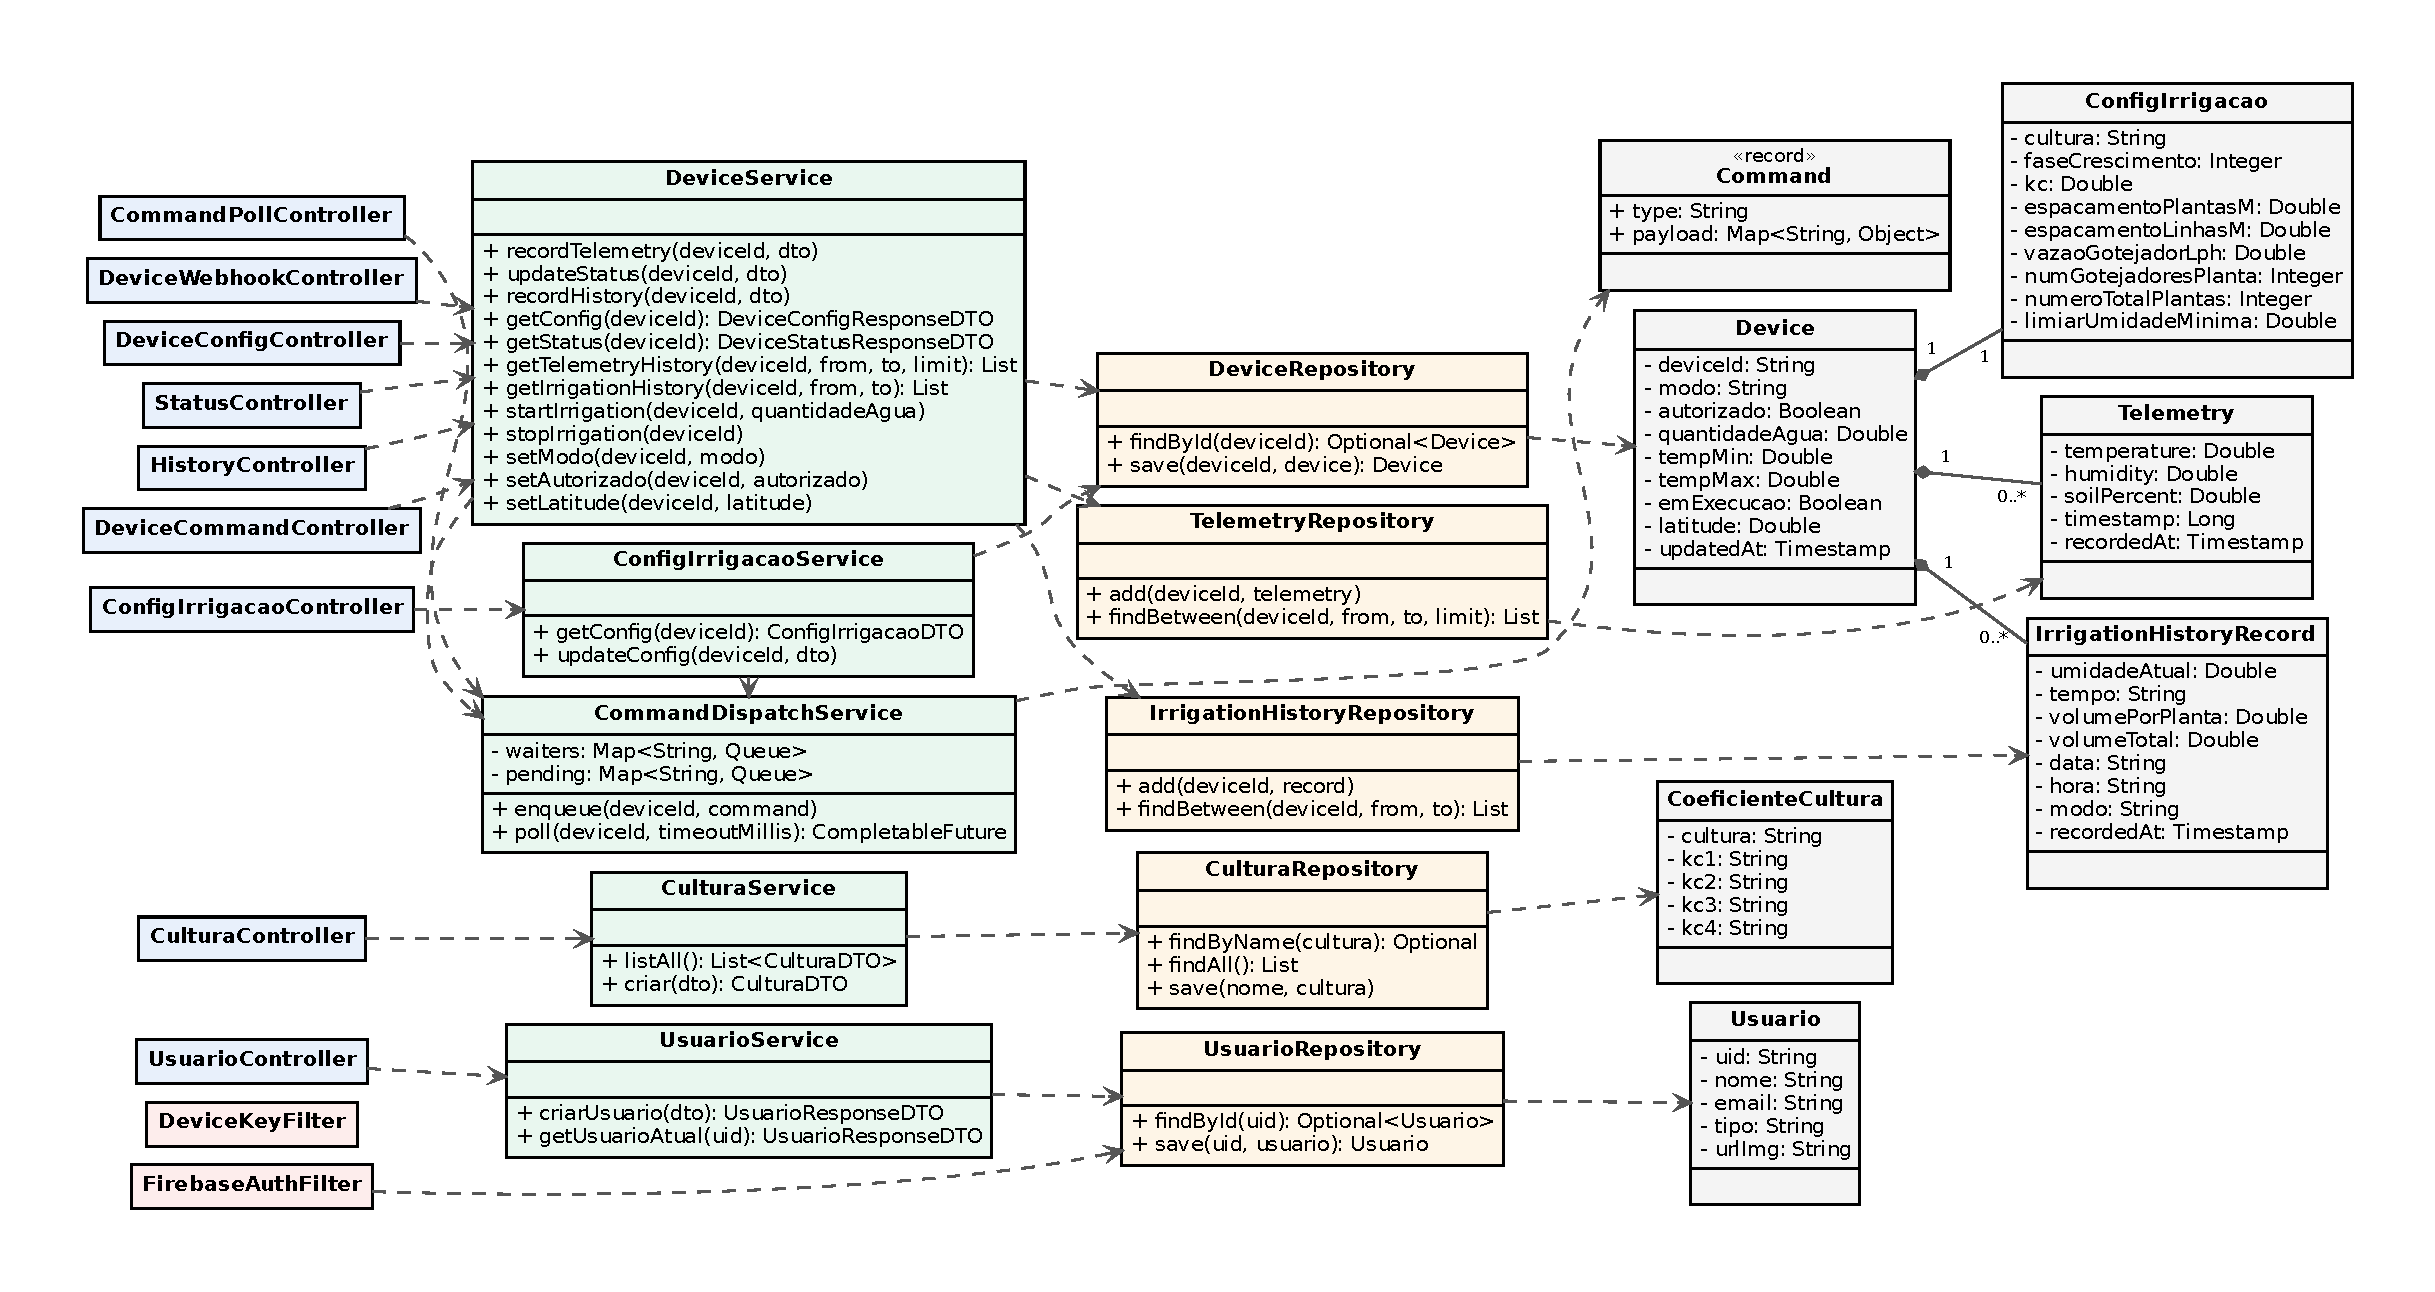
\includegraphics[width=\linewidth]{figuras/diagrama-classes-backend.pdf}
  \caption{Diagrama de classes do backend}
  \label{fig:classes-backend}
  \fonte{Elaborado pelo autor}
\end{figure}
\end{landscape}
}

\subsection{Endpoints e comunicação com o dispositivo}
\label{subsec:endpoints}

A Tabela~\ref{tab:endpoints} apresenta as rotas da API, separadas pelo cliente que as utiliza. Todas as rotas do painel que alteram o estado do sistema enfileiram um comando para o dispositivo, além de atualizar o Firestore.

{\small
\renewcommand{\arraystretch}{1.15}
\begin{longtable}{>{\raggedright\arraybackslash}p{1.4cm}
                  >{\raggedright\arraybackslash}p{7.3cm}
                  >{\raggedright\arraybackslash}p{5.9cm}}
  \caption{Rotas da API}
  \label{tab:endpoints} \\
  \hline
  \textbf{Método} & \textbf{Rota} & \textbf{Função} \\
  \hline
  \endfirsthead
  \multicolumn{3}{l}{Continuação da Tabela~\ref{tab:endpoints}} \\
  \hline
  \textbf{Método} & \textbf{Rota} & \textbf{Função} \\
  \hline
  \endhead
  \hline
  \multicolumn{3}{r}{Continua na próxima página} \\
  \endfoot
  \hline
  \endlastfoot
  \multicolumn{3}{l}{\textbf{Dispositivo (autenticado pela chave X-Device-Key)}} \\
  \hline
  POST & \texttt{/api/webhooks/telemetry} & Registra uma leitura dos sensores \\
  POST & \texttt{/api/webhooks/status} & Atualiza o estado do dispositivo \\
  POST & \texttt{/api/webhooks/history} & Registra uma irrigação concluída \\
  GET & \texttt{/api/devices/\{id\}/config} & Devolve a configuração inicial \\
  GET & \texttt{/api/devices/\{id\}/commands/poll} & Aguarda até 30~s por um comando (long-polling) \\
  \hline
  \multicolumn{3}{l}{\textbf{Painel (autenticado pelo Firebase; escrita só para o Administrador/Operador)}} \\
  \hline
  GET & \texttt{/api/devices/\{id\}/status} & Estado atual do dispositivo \\
  GET & \texttt{/api/devices/\{id\}/telemetry} & Leituras de um período (padrão: últimas 24~h) \\
  GET & \texttt{/api/devices/\{id\}/irrigation-history} & Irrigações de um período (padrão: últimos 30 dias) \\
  GET & \texttt{/api/devices/\{id\}/config-irrigacao} & Parâmetros agronômicos atuais \\
  PUT & \texttt{/api/devices/\{id\}/config-irrigacao} & Altera os parâmetros (\texttt{CONFIG\_IRRIGACAO}) \\
  PUT & \texttt{/api/devices/\{id\}/mode} & Troca o modo (\texttt{MODE\_CHANGE}) \\
  PUT & \texttt{/api/devices/\{id\}/authorization} & Autoriza ou bloqueia a irrigação automática (\texttt{AUTHORIZATION\_CHANGE}) \\
  PUT & \texttt{/api/devices/\{id\}/latitude} & Altera a latitude (\texttt{LATITUDE}) \\
  POST & \texttt{/api/devices/\{id\}/irrigation/start} & Inicia a irrigação manual (\texttt{START\_IRRIGATION}) \\
  POST & \texttt{/api/devices/\{id\}/irrigation/stop} & Interrompe a irrigação (\texttt{STOP\_IRRIGATION}) \\
  GET & \texttt{/api/culturas} & Lista as culturas e seus K$_c$ \\
  POST & \texttt{/api/culturas} & Cadastra uma cultura \\
  GET & \texttt{/api/usuarios/me} & Perfil do usuário autenticado \\
  POST & \texttt{/api/usuarios} & Cadastra um usuário \\
\end{longtable}
}
\vspace{-0.8\baselineskip}
\fonte{Elaborado pelo autor}

O principal desafio da comunicação foi entregar comandos a um dispositivo que está atrás da rede local do usuário e, portanto, não pode receber conexões vindas da internet. A solução adotada foi o long-polling: o ESP32 faz uma requisição à rota de comandos, e a API só responde quando há um comando para ele ou quando se passam 30~s sem comandos, caso em que devolve o código 204 (sem conteúdo). Em seguida, o dispositivo abre uma nova requisição. Com isso, um comando chega ao dispositivo quase imediatamente quando há uma consulta aberta, e em no máximo cerca de 30~s no pior caso (RNF06), sem que o ESP32 precise consultar a API a todo instante.

Na API, esse mecanismo é implementado pela classe CommandDispatchService, apresentada no Quadro~\ref{lst:dispatch}. Quando o dispositivo consulta a rota, o método poll devolve imediatamente um comando já pendente ou deixa a requisição registrada à espera, com um prazo de 30~s. Quando o painel gera um comando, o método enqueue o entrega à requisição que está esperando ou, se não houver nenhuma, guarda-o em uma fila para a próxima consulta. Do lado do controlador, a resposta é devolvida de forma assíncrona com a classe DeferredResult do Spring, o que libera a thread do servidor enquanto o dispositivo aguarda.

\noindent\begin{minipage}{\linewidth}
\begin{lstlisting}[language=Java, caption={Entrega de comandos por long-polling (trecho de CommandDispatchService)}, label={lst:dispatch}]
public void enqueue(String deviceId, Command command) {
    var queue = waiters.get(deviceId);
    if (queue != null) {
        CompletableFuture<Optional<Command>> waiting;
        while ((waiting = queue.poll()) != null) {
            if (waiting.complete(Optional.of(command))) {
                return; // entregue a uma consulta que estava aberta
            }
        }
    }
    // nenhuma consulta aberta: guarda para a proxima
    pending.computeIfAbsent(deviceId, id -> new ConcurrentLinkedQueue<>()).add(command);
}

public CompletableFuture<Optional<Command>> poll(String deviceId, long timeoutMillis) {
    var pendingQueue = pending.get(deviceId);
    Command alreadyPending = (pendingQueue == null) ? null : pendingQueue.poll();
    if (alreadyPending != null) {
        return CompletableFuture.completedFuture(Optional.of(alreadyPending));
    }
    var future = new CompletableFuture<Optional<Command>>();
    var queue = waiters.computeIfAbsent(deviceId, id -> new ConcurrentLinkedQueue<>());
    queue.add(future);
    timeoutExecutor.schedule(() -> {          // sem comando em 30 s: resposta vazia (204)
        if (future.complete(Optional.empty())) {
            queue.remove(future);
        }
    }, timeoutMillis, TimeUnit.MILLISECONDS);
    return future;
}
\end{lstlisting}
\vspace{-0.5\baselineskip}
\fonte{Elaborado pelo autor}
\end{minipage}
\medskip

\subsection{Segurança e autenticação}

A API usa dois mecanismos de autenticação, um para cada cliente, configurados com o Spring Security. O dispositivo envia em todas as requisições uma chave fixa no cabeçalho X-Device-Key, conferida pelo filtro DeviceKeyFilter (Quadro~\ref{lst:devicekey}). A chave é lida de uma variável de ambiente e nunca aparece no código-fonte (RNF03); requisições às rotas do dispositivo sem a chave correta recebem o código 401.

\noindent\begin{minipage}{\linewidth}
\begin{lstlisting}[language=Java, caption={Verificação da chave do dispositivo (trecho de DeviceKeyFilter)}, label={lst:devicekey}]
String cleanedUri = StringUtils.cleanPath(request.getRequestURI());
if (!DevicePaths.matches(cleanedUri)) {      // rota do painel: segue adiante
    filterChain.doFilter(request, response);
    return;
}
String key = request.getHeader("X-Device-Key");
if (key == null || !key.equals(firebaseEnv.deviceApiKey())) {
    response.sendError(HttpServletResponse.SC_UNAUTHORIZED, "X-Device-Key ausente ou invalida");
    return;
}
filterChain.doFilter(request, response);
\end{lstlisting}
\vspace{-0.5\baselineskip}
\fonte{Elaborado pelo autor}
\end{minipage}
\medskip

O usuário do painel faz login diretamente no Firebase Authentication, com e-mail e senha, e recebe um token que o painel envia no cabeçalho Authorization de cada requisição. O filtro FirebaseAuthFilter valida esse token com o Firebase Admin SDK e procura o usuário na coleção usuarios, que funciona como lista de acesso: quem não está cadastrado recebe o código 403, mesmo tendo uma conta válida no Firebase. O campo tipo do cadastro define o papel do usuário, como mostra o Quadro~\ref{lst:papel}. As rotas que alteram o sistema são marcadas com a anotação \texttt{@PreAuthorize("hasRole('ADMIN')")}, de modo que a restrição de escrita ao perfil Administrador/Operador (RN19) é verificada na própria API, e não apenas escondida no painel.

\noindent\begin{minipage}{\linewidth}
\begin{lstlisting}[language=Java, caption={Definição do papel do usuário (trecho de FirebaseAuthFilter)}, label={lst:papel}]
FirebaseToken token = firebaseAuth.verifyIdToken(header.substring("Bearer ".length()));
Usuario usuario = usuarioRepository.findById(token.getUid()).orElse(null);
if (usuario == null) {                       // fora da lista de acesso
    response.sendError(HttpServletResponse.SC_FORBIDDEN, "Usuario nao autorizado");
    return;
}
GrantedAuthority authority = new SimpleGrantedAuthority(
        "Administrador".equals(usuario.getTipo()) ? "ROLE_ADMIN" : "ROLE_USER");
\end{lstlisting}
\vspace{-0.5\baselineskip}
\fonte{Elaborado pelo autor}
\end{minipage}
\medskip

A autenticação do painel pode ser desligada pela variável de ambiente DASHBOARD\_AUTH\_ENABLED, recurso usado durante o desenvolvimento para testar as telas sem login. % CONFERIR: deixar DASHBOARD_AUTH_ENABLED=true na versão avaliada
O cadastro de novos usuários também passa pela API: o administrador preenche o formulário no painel, e a API cria a conta no Firebase Authentication e o registro correspondente na coleção usuarios, sem encerrar a sessão de quem está cadastrando.

\subsection{Modelo de dados}
\label{subsec:modelo-dados}

Os dados são armazenados no Cloud Firestore, banco NoSQL orientado a documentos \cite{firestore2026}. A Tabela~\ref{tab:colecoes} apresenta as coleções criadas. Cada dispositivo é um documento da coleção devices, identificado pelo seu nome (esp32-01), e as suas leituras e irrigações ficam em subcoleções desse documento. Essa organização acompanha a forma como os dados são consultados, sempre por dispositivo e por período, e permite incluir novos dispositivos sem alterar a estrutura (RNF17).

\begin{table}[htbp]
  \centering
  \caption{Coleções do Cloud Firestore}
  \label{tab:colecoes}
  \small
  \renewcommand{\arraystretch}{1.2}
  \begin{tabularx}{\textwidth}{>{\raggedright\arraybackslash}p{6.3cm}
                               >{\raggedright\arraybackslash}X}
    \hline
    \textbf{Coleção} & \textbf{Conteúdo de cada documento} \\
    \hline
    \texttt{devices} & Estado do dispositivo (modo, autorização, volume de água, temperaturas mínima e máxima, irrigação em andamento, latitude) e os parâmetros agronômicos: cultura, fase, K$_c$, espaçamentos, vazão e número de gotejadores, número de plantas e limiar de umidade \\
    \texttt{devices/\{id\}/telemetry} & Uma leitura: temperatura e umidade do ar, umidade do solo e data e hora do registro \\
    \texttt{devices/\{id\}/irrigationHistory} & Uma irrigação: umidade antes, tempo, volume por planta, volume total, data, hora e modo \\
    \texttt{coeficientes} & Uma cultura e o seu K$_c$ em cada uma das quatro fases (kc1 a kc4) \\
    \texttt{usuarios} & Um usuário autorizado: nome, e-mail e tipo (Administrador ou Visualizador) \\
    \hline
  \end{tabularx}
  \fonte{Elaborado pelo autor}
\end{table}

As consultas de histórico filtram as leituras pela data de gravação, ordenam-nas da mais recente para a mais antiga e devolvem no máximo um número fixo de documentos: 500 por padrão, ou o limite pedido pelo cliente, que na tela de histórico é de 2.000. Esse limite mantém o tempo de resposta estável mesmo com o acúmulo de dados, já que, com leituras a cada 10~s, cada dia gera cerca de 8.640 documentos.

% =====================================================================
\section{Frontend}
\label{sec:frontend}

O painel web foi desenvolvido em Angular 21, com componentes independentes (standalone) e signals para manter o estado da tela atualizado. A estilização usa o Tailwind CSS, os gráficos usam o Chart.js e o login usa o SDK JavaScript do Firebase.

\subsection{Estrutura da aplicação}

O código é dividido em duas pastas principais. A pasta core reúne o que é compartilhado entre as telas: os modelos de dados, os serviços que acessam a API, os guards que protegem as rotas e os interceptadores de requisições. A pasta features reúne as telas, cada uma com os seus próprios componentes, carregadas sob demanda na primeira vez em que são abertas.

O serviço IrrigationService concentra a comunicação com a API. Ele consulta o estado do dispositivo a cada 5~s e as leituras dos sensores a cada 10~s (RNF05) e guarda os resultados em signals, de modo que todas as telas exibem os mesmos dados sem fazer requisições repetidas. Após uma ação do usuário, como iniciar uma irrigação, o serviço antecipa a próxima consulta para que a tela reflita a mudança logo em seguida.

O acesso às telas é controlado por dois guards: o authGuard exige que o usuário esteja autenticado, e o adminGuard libera as telas de cadastro de usuários e de culturas apenas para o Administrador/Operador. Dois interceptadores atuam em todas as requisições à API: o primeiro anexa o token do Firebase ao cabeçalho Authorization (Quadro~\ref{lst:interceptor}), e o segundo encerra a sessão e volta à tela de login quando a API responde com os códigos 401 ou 403. Para o desenvolvimento, o painel também pode funcionar com dados simulados, sem depender da API (RNF11).

\noindent\begin{minipage}{\linewidth}
\begin{lstlisting}[language={}, caption={Inclusão do token nas requisições à API (auth.interceptor.ts)}, label={lst:interceptor}]
export const authInterceptor: HttpInterceptorFn = (req, next) => {
  if (!req.url.startsWith(environment.apiBaseUrl)) {
    return next(req);                 // requisicoes externas seguem sem token
  }
  const auth = inject(AuthService);
  return from(auth.getIdToken()).pipe(
    switchMap((token) => {
      const authorizedReq = token
        ? req.clone({ setHeaders: { Authorization: `Bearer ${token}` } })
        : req;
      return next(authorizedReq);
    }),
  );
};
\end{lstlisting}
\vspace{-0.5\baselineskip}
\fonte{Elaborado pelo autor}
\end{minipage}
\medskip

\subsection{Telas desenvolvidas}

O painel possui seis telas, descritas a seguir. As Figuras~\ref{fig:tela-login} a~\ref{fig:tela-cadastro} mostram cada uma delas.

A tela de login (Figura~\ref{fig:tela-login}) recebe o e-mail e a senha e autentica o usuário no Firebase; em seguida, o painel busca o perfil do usuário na API para saber quais ações liberar.

\begin{figure}[htbp]
  \centering
  % Troque a linha abaixo por: \includegraphics[width=0.8\textwidth]{figuras/tela-login}
  \figuraprovisoria{6cm}{Inserir captura da tela de login}
  \caption{Tela de login}
  \label{fig:tela-login}
  \fonte{Elaborado pelo autor}
\end{figure}

O dashboard (Figura~\ref{fig:tela-dashboard}) é a tela principal. Ele mostra o estado do dispositivo e as últimas leituras dos sensores, permite alternar entre os modos manual e automático, autorizar ou bloquear a irrigação automática, iniciar e interromper a irrigação manual com o volume em litros, acompanhar o tempo restante de uma irrigação em andamento e consultar os dados da última irrigação e os parâmetros agronômicos em uso. Para o Visualizador, os controles aparecem desabilitados.

\begin{figure}[htbp]
  \centering
  % Troque a linha abaixo por: \includegraphics[width=\textwidth]{figuras/tela-dashboard}
  \figuraprovisoria{8cm}{Inserir captura do dashboard}
  \caption{Tela principal (dashboard)}
  \label{fig:tela-dashboard}
  \fonte{Elaborado pelo autor}
\end{figure}

A tela de histórico (Figura~\ref{fig:tela-historico}) apresenta gráficos da temperatura do ar, da umidade do ar e da umidade do solo nos períodos de 24 horas, 7 dias e 30 dias, e uma tabela com as irrigações realizadas.

\begin{figure}[htbp]
  \centering
  % Troque a linha abaixo por: \includegraphics[width=\textwidth]{figuras/tela-historico}
  \figuraprovisoria{8cm}{Inserir captura da tela de histórico}
  \caption{Tela de histórico}
  \label{fig:tela-historico}
  \fonte{Elaborado pelo autor}
\end{figure}

A tela de configurações (Figura~\ref{fig:tela-configuracoes}) reúne a latitude da área e os parâmetros agronômicos. O usuário escolhe a cultura e a fase de desenvolvimento, e o K$_c$ correspondente é aplicado automaticamente a partir do catálogo, sem ser digitado (RN13).

\begin{figure}[htbp]
  \centering
  % Troque a linha abaixo por: \includegraphics[width=\textwidth]{figuras/tela-configuracoes}
  \figuraprovisoria{8cm}{Inserir captura da tela de configurações}
  \caption{Tela de configurações}
  \label{fig:tela-configuracoes}
  \fonte{Elaborado pelo autor}
\end{figure}

Por fim, duas telas são exclusivas do Administrador/Operador: a de cadastro de culturas (Figura~\ref{fig:tela-cultura}), em que se informam o nome da cultura e o K$_c$ de cada uma das quatro fases, e a de cadastro de usuários (Figura~\ref{fig:tela-cadastro}), em que se informam o nome, o e-mail, a senha inicial e o perfil do novo usuário.

\begin{figure}[htbp]
  \centering
  % Troque a linha abaixo por: \includegraphics[width=0.8\textwidth]{figuras/tela-nova-cultura}
  \figuraprovisoria{6cm}{Inserir captura da tela de cadastro de culturas}
  \caption{Tela de cadastro de culturas}
  \label{fig:tela-cultura}
  \fonte{Elaborado pelo autor}
\end{figure}

\begin{figure}[htbp]
  \centering
  % Troque a linha abaixo por: \includegraphics[width=0.8\textwidth]{figuras/tela-cadastro}
  \figuraprovisoria{6cm}{Inserir captura da tela de cadastro de usuários}
  \caption{Tela de cadastro de usuários}
  \label{fig:tela-cadastro}
  \fonte{Elaborado pelo autor}
\end{figure}
